\chapter{Phonology}
\label{ChapterPhon}
	
There are 55 phonemes; 20 phonemic vowels (5 qualities, length and nasality are contrastive) and 35 consonants. The number of both consonant and vowel phonemes puts the phoneme inventory of Vamale in the top 10\% on Phoible (with ca. 3000 compared inventories) \parencite{phoible}, and in the second-largest group of the sample studied by Maddieson et. al in \citetitle{wals}, which assigns it a high consonant-to-vowel quality ratio.\footnote{Note that this counts vowel qualities but not contrastive quantity, hence 35 consonants\slash 5 vowels  yielding a ratio of 7.}
The emphasis on consonants is typical of the Northern and Far Northern languages, and was not diminished by the proximity of consonant-poorer Cèmuhî, nor was it substantially enriched by Pije, which has e.g. /ɾ̥/.
	
	
\section{Transcription}
\is{Transcription}
Following the transcription system established by \textcite{ozanne-rivierre_phonologie_1982}% (\textbf{Could you say whether this system is rather broad or narrow, i.e. rather phonemic or phonetic? Your pre-nasalized segments in this paragraph and Table 1.1 suggest the latter...})
, this work will use \ort{h} after plosives to mark aspiration (regardless of its phonemic status), \ort{h} before nasals and liquids to mark voicelessness, and the circumflex diacritic to mark nasal quality in vowels (see \Cref{tab:transcr_system} for an overview). All voiced plosives are typically pre-nasalized%, a feature inherited from Proto-Oceanic
: /ᵐb/, /ⁿd/, /ⁿɟ/, /ᵑg/. This is systematic and, following the local linguistic tradition, will not be represented. Vowels are nasalized after nasals, and often also before them (this includes the pre-nasal elements in voiced plosives such as /ᵐb/, to an extent). There is also interplay with aspirated plosives for historical reasons  (see \sectref{ssec:Aspiration}). Only phonemically nasal vowels will be represented as nasal, with the circumflex diacritic \ort{\^{}} used in all Northern transcription systems. Compare the representations of (\ref{ex:nasal}) with phonemic nasalization with (\ref{ex:nasal2}) with predictable aspiration.
	\is{Vowels!Nasal vowels}
	
	
	\ea \label{ex:nasal}
		[wĩ̃ːn jeː]\\
		\gll wîî-n yee\\
		 strength-\gl{nspec}.\gl{poss} tree\\
		\glt \qu{strength of a tree}
		\z
		
		
		\ea \label{ex:nasal2}
		[wĩːn jeː]\\
		\gll wii-n yee\\
		 field-\gl{nspec}.\gl{poss} tree\\
		\glt \qu{orchard}
	\z  



True minimal pairs between oral and phonemic nasal vowels are rare, while contexts in which phonemically oral vowels are nasalized abound. The degree of nasality depends on the speaker, so the phonetic difference depicted in example (\ref{ex:nasal}) is not a representative or reliable criterion to identify phonemically nasal vowels, though the latter tend to be more strongly nasal than nasalized ones. %Since phonemic status is not always clearly determined, circumflex diacritics will also mark nasal vowels where the nasal quality is not necessarily phonologically conditioned, as for \ort{phwê} /pʰʷɛ̃/ \qu{moon} (see \sectref{ssec:Aspiration} and \sectref{ssec:NasalV}).
	
%	\begin{table}
%		
%		\centering
%		\caption{Transliteration system used in this thesis}
%		\label{tab:transcr_system}
%		\begin{tabular}{l|llllllllllllllllll}
%		Aspirated Plosives&  \ort{phw}& /pʰʷ/& \ort{ph} & /pʰ/ & 	\ort{th}& /tʰ/& \ort{ch}&[cʰ]&\ort{kh}&/kʰ/&&&&&&&& \\
%		Tenuis Plosives& \ort{p} & /p/ & \ort{t}& /t/ & \ort{c} & /c/ & \ort{k} & /k/ &&&&&&&&&&\\
%		Voiced Plosives& \ort{b}& /ᵐb/&\ort{bw}& /ᵐbʷ/& \ort{j}& /ⁿɟ/ & \ort{g} & /ᵑɡ/ &&&&&&&&&&\\
%		
%		Nasals& \ort{m} /m/ &  \ort{hm}& /m̥/& \ort{n} & /n/ & \ort{hn} & /n̥/ &\ort{ny}& /ɲ/& \ort{hny}& /ɲ̊/ & \ort{ng} & /ŋ/ &  \ort{hng} & /ŋ̊/ &&&\\
%		Fricatives & \ort{f}  /f/ & \ort{fw}  /fʷ/ & \ort{v}  /v/ & vw & /vʷ/ & \ort{s}& /s/&	\ort{xh}& /x/&	\ort{x} & /ɣ/ & xw & /xʷ/ & \ort{h} & /h/ &&&\\
%		Approximants & \ort{l}  /l/ & \ort{hl} & /l̥/ & \ort{w} & /w/ & \ort{y} & /j/ & \ort{hy}& [ç] \goodtilde [j̥]&&&&&&&&&\\
%		Vowels&	\ort{i}  /i/ &	\ort{ii}& /iː/ & \ort{î}& /ĩ/ & \ort{îî} & /ĩː/&\ort{e}&[e] \goodtilde [ɛ] & \ort{ê} & /ɛ̃/&\ort{o}& [o] \goodtilde [ɔ]&\ort{ô} & /ɔ̃/&&&\\
%	
%		\end{tabular}
%	\end{table}

	\begin{table}
	\caption{Transliteration system used in this book}
	\label{tab:transcr_system}

	\begin{tabular}{llllll}
	\lsptoprule
		  \ort{ph} /pʰ/ &  \ort{phw} /pʰʷ/&	\ort{th} /tʰ/& \ort{ch} [cʰ]&\ort{kh} /kʰ/ \\
		\ort{p}  /p/ &\ort{pw}  /pʷ/& \ort{t} /t/ & \ort{c}  /c/ & \ort{k}  /k/ \\
		\ort{b} /ᵐb/&\ort{bw} /ᵐbʷ/& \ort{d} /ⁿd/&\ort{j} /ⁿɟ/ & \ort{g}  /ᵑɡ/ &\\
		  \ort{hm} /m̥/& \ort{hmw} /m̥ʷ/& \ort{hn}  /n̥/ & \ort{hny} /ɲ̊/ &   \ort{hng}  /ŋ̊/ \\
	\ort{m} /m/&	\ort{mw} /mʷ/ & \ort{n}  /n/ &  \ort{ny} /ɲ/& \ort{ng} /ŋ/ \\
		\midrule
		 \ort{f}  /f/ & \ort{fw}  /fʷ/ & \ort{s} /s/&	\ort{xh} /x/& \ort{xw}  /xʷ/ & \ort{h}  /h/ \\
		  \ort{v} /v/ & \ort{vw}  /vʷ/ &&	\ort{x}  /ɣ/&& \\
&&	\ort{l}  /l/ & \ort{y}  /j/ & \ort{w}  /w/ &\\
&&	\ort{hl}  /l̥/ & \multicolumn{2}{l}{\ort{hy} [ç] \goodtilde [j̥]}&\\
	\midrule
	\ort{i}  /i/ &&	\ort{ii} /iː/ &&&\\
	 \ort{î} /ĩ/ && \ort{îî}  /ĩː/&&&\\
	 \ort{e} [e] \goodtilde [ɛ] &\ort{ee} [eː] \goodtilde [ɛː] &&&\\
	  \ort{ê} /ɛ̃/&&\ort{êê}  /ɛ̃ː/&&&\\
	  \ort{o} [o] \goodtilde [ɔ]&\ort{oo} [oː] \goodtilde [ɔː]&&&\\
	  \ort{ô}  /ɔ̃/&&\ort{ôô}  /ɔ̃ː/&&&\\
		\lspbottomrule
	\end{tabular}
\end{table}


	\begin{sloppypar}
	Vamale speakers frequently code-switch to French. Established loanwords such as \textit{watuut} \qu{car} are transcribed according to the system in \Cref{tab:transcr_system}, whereas \textit{ad hoc} loans are written as they would be in French and italicized to help distinguish them from older Vamale words (\ref{ex:devoirs}).
	\end{sloppypar}
	
	\ea \label{ex:devoirs}
		\gll tha le=vwa \textit{devoirs}-le\\
			  \gl{ass} 3\gl{pl}=do homework-3\gl{pl}.\gl{poss}\\
		\glt \qu{They do their homework.}
	\z\index[gls]{ass}
	
	\section{Consonants}
	\label{sec:consphonemes}
	\is{Consonants}
	The consonants, shown in \Cref{tab:cons}, can be classified along two axes: aspiration (aspirated vs. non-aspirated) and nasality (nasal vs. semi-nasal vs. oral). This has historical reasons, as will be shown in \sectref{sec:phonhist_dev}. 
	While all consonants may appear word-initially and between vowels, a historical neutralization has reduced the set of syllable-final ones: /p, t, tɕ, k, m, n, ɲ, ŋ/, i.e. simple voiced nasals and voiceless plosives. Syllable-final /k/, /tɕ/ and /ɲ/ are much rarer than the others and are undergoing mergers with /ʔ/, /t/, and /n/ respectively. 
	\begin{itemize}
		
	\item /piuk/ \qu{spark} $\rightarrow$ [ˈpiˑ.uʔ] 
	\item /jilowec/ \qu{tree sp.} $\rightarrow$  [ⁿɟi.ˈlo.wɛt] 
	\item /waɲ/ \qu{consequence of taboo breaking} $\rightarrow$ [wan])

\end{itemize}
	 /k/ and /tɕ/ are often simply dropped. The deletion of final consonants is a sound change that is described as affecting mountain Voh-Koné varieties \parencite[25]{campbell_phenomenon_1987}, and is furthest advanced in the coastal variety of Vamale. This final consonant deletion only concerns inherited lexemes, since numerous loanwords from French and Kanak languages feature other syllable-final consonants (\textit{bagaas} \qu{luggage}, \textit{cakes} \qu{\gl{expl}}).
	While syllable-final /k/ is often dropped, /k/ is also rare in syllable onsets: many words with k- are either loans or grammatical terms, e.g. \textit{ka} \qu{\gl{sbj}}, \textit{ka} \qu{\gl{cnj}}, \textit{ko} \qu{obl}, \textit{-ke} \qu{\gl{tr}}, \textit{kai} \qu{who?}, \textit{kacahô} \qu{rather than}, \textit{kavi} \qu{but}. Lexical, apparently non-borrowed words number fewer than 10 items in the recorded dictionary. While a historical sound change lenited *k- to ɣ- (see \sectref{sec:quesphon}), explaining the rarity of \textit{k}-, it is noteworthy that many words that retained initial k- are grammatical terms.
	
	Vamale consonants distinguish a voiceless series from a pre-nasalized voiced series. This is a feature retained from Proto-Oceanic, and not widespread east of New Caledonia \parencite[196--197]{ozanne-rivierre_proto-oceanic_1992}. A typical feature of Northern New Caledonian is the presence of labio-velar plosives and fricatives, and voiceless nasals and liquids. Labio-velarized consonants do not precede /u/ and /o/ for historical reasons: one element merged into the other.

	\begin{table}
		\caption{Consonants in Vamale. Non-phonemes are in brackets.}
		\begin{tabular}{ *6{l} }
			\lsptoprule
			             & Bilabial & Lab. Bilab. & Labiod. & Lab. Labiod. \\\midrule
			Plosive      & pʰ p ᵐb & (pʰʷ) pʷ ᵐbʷ &         &              \\
			Nasal        & m̥ m     & m̥ʷ mʷ        &         &            \\
			Tap          &         &              &         &              \\
			Fricative    &         &              & f v     & fʷ vʷ        \\
			Approximant  &         &              &         &              \\
			Lat. Approx. &         &              &         &              \\\midrule
			             & Alveolar & Palatal & Velar & Lab. Velar & Glott. \\\midrule
             Plosive     & tʰ t ⁿd & (cʰ) c ⁿɟ & kʰ k ᵑɡ  &    &  \\
             Nasal       & n̥ n     & ɲ̊ ɲ       & (ŋ̊) ŋ    &    &  \\
             Tap         & (ɾ)     &           &          &    &  \\
             Fricative   & s       &           & x ɣ      & xʷ & h \\
             Approximant &         & j         &          & w  &  \\
             Lat. Approx.& l l̥     &           &          &    &\\
			\lspbottomrule
		\end{tabular}
		\label{tab:cons}
	\end{table}

	\subsection{Examples}
	A table listing examples in word-initial, -internal, and -final positions is given in \Cref{tab:consex}. No study was done on the frequency of the phonemes, but some consonants are much rarer than others. Syllable-final /k/ has all but disappeared in a regular sound-change, and occurs only in loans from Pije and other languages: e.g. \textit{piuk} \qu{nail}\footnote{POc *pituqun, \textit{piguk} \qu{star} in Nêlêmwa \parencite[21]{bril_nelemwa_2002}.} and \textit{xhwahyuk} \qu{whistle} are originally Pije. %It is noteworthy that Campbell described this apocope as even more complete for Vamale, with \textit{piu} \qu{star} (normally \textit{xhafuthiin} in coastal Vamale, but \textit{daan-piuk} \qu{thorn-spark; nail}) \parencite[120]{campbell_phenomenon_1987}. 
%	Syllable-final /c/ is similarly on its way out, and final /ɲ/, lacking contrastive contexts, seems to merge with /n/. 
	/r/ only occurs in loans. Initial /ŋ/ is probably a loan phone from Pije, given that it only appears in one plant species name (\textit{ngeein}), and is in free variation with \textit{mwangin} \goodtilde \textit{ngangin} \qu{sour}. Finally, all aspirated plosives except /tʰ/ are rare.
	
	\begin{table}
		\caption{Examples showing Vamale consonants in monomorphemic words.}
	\small
	\resizebox{.85\textwidth}{!}{
		\begin{tabular}{l *3{l@{~}l} }
			\lsptoprule
			& \multicolumn{2}{l}{Initial} & \multicolumn{2}{l}{Medial} & \multicolumn{2}{l}{Final}\\\midrule
			\multicolumn{7}{l}{Plosives}  \\
			&   \textit{pwan}& \qu{on} & \textit{sapwen}& \qu{clothing} &&\\
			&	\textit{phwaat}& \qu{clear} & \textit{xhwaaphwê}& \qu{araucaria sp.} & &\\
			&	\textit{bwan}& \qu{head} & \textit{siibwi}& \qu{rat} & & \\
			&	\textit{pa}& \qu{\gl{prf}} & \textit{ape}-& \qu{trace} & \textit{thap}& \qu{pandanus} \\
			&	\textit{phuake}& \qu{prod} &  &&&\\
			&	\textit{ba}& \qu{wall} & \textit{abu}& \qu{1\gl{du}.\gl{excl}} & &\\
			&	\textit{thake} & \qu{throw} &  \textit{mathila}& \qu{bird sp}& &\\
			&	\textit{ta}& \qu{go up} & \textit{mata}& \qu{sing} & \textit{fuut}& \qu{whistle} \\
			&	\textit{da}& \qu{spear} & \textit{udu}& \qu{drink} & &\\
			&	\textit{cabi}& \qu{break} & \textit{kicaa}& \qu{jealous} & \textit{tuuc}& \qu{take out} \\
			&	\textit{jigo}& \qu{mangrove} & \textit{vije}& \qu{bird snare} & & \\
			&	\textit{ka}& \qu{\gl{sbj}} & \textit{buke}& \qu{flower} & \textit{piuk}& \qu{spark} \\
			&	\textit{gi}& \qu{adze} & \textit{hagu}& \qu{snake} & &\\
			\midrule
			\multicolumn{7}{l}{Fricatives, glides, and liquids} \\
			&   \textit{fuu}& \qu{wash} & \textit{fufudo} & \qu{foam} &&\\
			&	\textit{vaa}& \qu{war} & \textit{fava}& \qu{four}&&\\
			&	\textit{fwa}& \qu{hole} &  \textit{waafwap}& \qu{raven} && \\
			&	\textit{vwa}& \qu{do, have} & \textit{xhaavwa}& \qu{wait} & &\\
			&	\textit{siteke}& \qu{sacred} & \textit{gase}& \qu{1\gl{pl}.\gl{incl}} &&\\
			&	\textit{xhopwen}& \qu{big} & \textit{haxhi}& \qu{forgive} && \\
			&	\textit{xhwatin}& \qu{small} & \textit{sixhwe}& \qu{imitate} & & \\
			&	\textit{holeeke}& \qu{thank} & \textit{yahan}& \qu{leave} &&\\	
			&	\textit{xat}& \qu{sun} && && \\
			&	\textit{xhat} & \qu{clitoris} & \textit{bwaxhu}&\qu{hat} &&\\
			&	\textit{yatan}& \qu{name} & \textit{vaya}& \qu{work} & &\\
			&	\textit{wadan}& \qu{time} &   \textit{nyawan}& \qu{spirit} &&\\
			&	\textit{ra}-& \qu{\gl{reccont}} & \textit{gere}& \qu{fat} & &\\
			&	\textit{lu}& \qu{3\gl{du}} &\textit{pwalalu}& \qu{rainbow} & &\\
			&	\textit{hluupwi}& \qu{suck in} &\textit{bwahli}& \qu{long} & &\\
			\midrule	
			\multicolumn{7}{l}{Nasals} \\
			&	\textit{hmwet}& \qu{tired} & \textit{saahmwa}& \qu{banana} & &\\
			&	\textit{mwa}& \qu{house} & \textit{imwi}& \qu{grab}& & \\
			&	\textit{hma}& \qu{arrive} & \textit{cahma}& \qu{whereas} & & \\
			&	\textit{ma}& \qu{\gl{com}} & \textit{cama}& \qu{if} & \textit{xam}& \qu{mat}\\
			&	\textit{hnep}& \qu{sail} & \textit{ehni}& \qu{prox}& & \\
			&	\textit{naen}& \qu{now} & \textit{jinu}& \qu{power} & \textit{thiin} & \qu{close} \\
			&	\textit{hnyimake}& \qu{think} & \textit{bwihnyo} &\qu{clam}  & & \\
			&	\textit{nyau}& \qu{bad} & \textit{xhanyip}& \qu{dream} & \textit{wany}& \qu{punishment}\\
			&	\textit{ngein}& \qu{cycas sp.} & \textit{dingan}& \qu{creek} & \textit{vaang}& \qu{unknown} \\
		\lspbottomrule
		\end{tabular}
		}
		\label{tab:consex}
	\end{table}
	
%	\footnotetext{\gl{prf} }
	\subsection{Marginal phonemes}
	\label{sec:quesphon}
	
	\is{Marginal phonemes![ŋ̊]}
	Some segments appear rarely, are not produced by all speakers, or present a distribution which hints at (former) allophony. This affects most voiceless plosives, the tap \ort{r} [ɾ], the voiceless lateral approximant [l̥] and the voiceless velar nasal. \ort{hng} /ŋ̊/ only appears in \textit{jahngan} \qu{length}, and is in free variation with its voiced counterpart. Three factors indicate that /ŋ̊/ is a loan in this word: (a) the aspiration of nasals can be almost or completely inaudible (intervocalic nasals are more audibly aspirated than initial ones), (b) neither Bwatoo nor Hmwaveke seem to have it in any other words, and (c) only Western Nemi (no present-day contact) has it as a phoneme. 
	
	\is{Marginal phonemes![ɾ]}
	The tap \ort{r} [ɾ] is a phoneme in Nemi and in Fwâi \parencite[18; 19]{ozanne-rivierre_phonologie_1982}. It appears only in loanwords in Pije \parencite[17]{ozanne-rivierre_phonologie_1982} and Cèmuhî \parencite[21]{rivierre_langue_1980}, and does the same in Vamale. There is one instance where I recorded \ort{ra-} as an aspectual prefix \qu{to have been doing for a short while} in unelicited speech. I was able to contrast it with \ort{xa-} /ɣa/, compare examples \REF{ex:x} and \REF{ex:r}.
	
	\ea
	\label{ex:x}
		\gll a=xa-soom la\\	
	 3\gl{sg}=\gl{agt}.\gl{nmlz}-swim be.here\\
	\glt \qu{S/he usually swims here.}
	\z
	
	
	\ea\label{ex:r}
	\gll a=ra-xa-soom la\\
	 3\gl{sg}=\gl{reccont}-\gl{agt}.\gl{nmlz}-swim be.here\\	
	\glt \qu{S/he recently picked up the habit of swimming here.}
		\z
	
	\ort{ra-} is described for Bwatoo as a continuative particle, see example \REF{ex:Bwatoo_ra} \parencite[57]{rivierre_bwatoo_2006}, whereas \ort{xha} /xa/ is the habitual aspect marker (/ɣa-/ in Vamale). \textit{Ra} is not used in these contexts in Vamale (where the continuative marker is \textit{balan}). \textit{Ra} is probably a loan from the West Coast, and [ɾ] most likely a relatively free variant of /ɣ/, except in this one prefix \textit{ra-} \qu{\gl{reccont}}.
	
	\ea \label{ex:Bwatoo_ra}	
	\gll ka le ra vila na ni bee-le\\
	 \gl{cnj} 3\gl{pl} \textit{persist}. dance \gl{agt} \gl{def}.\gl{pl} peer-3\gl{pl}.\gl{poss}\\
	\glt \qu{The others keep dancing.}
	\z
	
	
	\ea	
	\gll a bwaa ra Numea\\	
	 3\gl{sg} \gl{ipfv} \textit{persist}. N.\\
		\glt \qu{S/he is still in Noumea.}	
	\z
	
	\is{Marginal phonemes![kʰ]}
The status of [kʰ] is tricky in the sense that, while both the aspirated and the non-aspirated phone exist, the aspirated one only very rarely occurs without a nasalized vowel following it. There are no minimal pairs with [k], and the few occurrences of [kʰ] before oral vowels are loanwords or due to fortis-spreading (see \sectref{ssec:Aspiration}). 

	\is{Marginal phonemes![pʰ]}
Bilabial voiceless plosives exist with aspiration and without, as well as with labiovelarization. So far, the origin of either remains to be established, as the regular sound changes reconstructed by \citeauthor{ozanne-rivierre_structural_1995} mostly led to the development of fricatives. [pʰ] is attested before the oral rounded vowels [u] and [o], and before nasal vowels. The latter are a sound class intimately related to aspiration, as is discussed in \sectref{ssec:Aspiration}. Most instances of [pʰ] before a nasal vowel may be produced with a velar fricative [pʰʷ] \goodtilde [pχ]. The glide [w] and rounded back vowels have merged in modern Vamale. There are no minimal pairs between [pʰ] and [pʰʷ]. There are no perfect minimal pairs with either and /p/, though this contrast is clearer, e.g. neither /p/ nor /pʷ/ precedes nasal vowels. Both /p/ and [pʰ] before oral back vowels are rare. The following words constitute the entirety of the types recorded in the lexicon, many of which are found in non-Voh-Koné languages as well: \begin{itemize}
\item \textit{pu} \qu{on the ground} \item \textit{puput} \qu{behind sth inanimate} \item \textit{phuake} \qu{wiggle} \item  \textit{poon} \qu{coconut fibre} \item \textit{phoop} \qu{snail}, \textit{phom} \qu{butterfly} \item \textit{pola} \qu{type of weaving} \item \textit{photha} \qu{sexual taboo; women's part of the village}\footnote{From \citegen{leenhardt_langues_1946} notes, not used nowadays.} 
\end{itemize}
Furthermore, there are no instances of /f/ and /fʷ/ followed by a nasal vowel, but many cases of /f/ before rounded back vowels. Hence, an imperfect distribution of labiodental fricatives and bilabial aspirated plosives can be identified: front and central vowels are only found after fricatives, nasal vowels only after plosives, and rounded back vowels can follow either. In conclusion, [pʰ] and [pʰʷ] may be former allophones of /f/ and /fʷ/ before nasal vowels, and [pʰ] is now present before oral vowels due to contact with other languages, perhaps Pije \parencite[518]{rivierre_contact_1994}. The unaspirated bilabial plosives were borrowed from neighboring languages as well \parencite[516]{rivierre_contact_1994}, or constitute remains of an incomplete sound change *p $\rightarrow$ \textit{v}. 
 %\todo{where is p and pw from?}
	%BUT: pu/puput, poon/pola/pook (loanwords?), pwa, etc. fuu, foovwat etc. 
	
	%xxFor these reasons, both [pʰ] and [kʰ] are old allophones of /p/ and /k/ in old Vamale words, and nowadays available loan phones in loanwords. 
	
	\subsection{Labio-velarized consonants}
	\is{Consonants!Labio-velarized consonants}
	Labio-velar consonants in Vamale are all labial (/ᵐbʷ/, /fʷ/, /mʷ/, etc), with the exception of /xʷ/. To explain this, Campbell suggests that /xʷ/ should be analyzed as an allophone or a surface realization of /w̥/ \parencite[37]{campbell_phenomenon_1987}, with /w̥/ as the fortis %couterpart to 
	/w/ (see \sectref{ssec:Aspiration} for an introduction to Vamale fortis). This makes sense as it makes the Hmwa(v)eke systems fit into their regional context, as voiceless liquids and glides are widespread in other Northern languages. 
		%\subsection{Pre-nasalized consonants}
	%Pre-nasals have bled into Kanak French, seems to intensify when people want to emphasize their Kanakdom.
	%Because a nasal followed by a voiced plosive at the same point of articulation ([nd],[mb],[nɟ],[ŋg]) could be viewed as a part of the plosive, there are no morpheme-final voiced plosives, except in loan words.
	
	\subsection{Voiceless nasals}
	\label{sec:phonhist_dev}
	\is{Consonants!Voiceless nasals}
	Every nasal except /ŋ/ has a fortis, i.e. voiceless counterpart, e.g. /m̥uːn/ \qu{smoke} vs /muːn/ \qu{blossom}. Like most of the aspirated plosives, voiceless nasals in Vamale have probably developed from forms that were reduplicated in POc and geminated in PNC, and which were perhaps already devoiced in Proto-North, for instance *nana(q) \qu{pus} $\rightarrow$	\textit{hnau-}\slash\textit{hnau-} \qu{snot} \parencite[27]{ozanne-rivierre_phonologie_1982}.

	In Bwatoo and in Vamale, the phonation of nasals and liquids can be influenced by the fortis status of other consonants in the surrounding syllables. Bwatoo examples include the following, with the triggering consonants in bold:
	
	\ea  \parencite[27]{rivierre_bwatoo_2006}
		\ea \textit{\textbf{f}omwa} \goodtilde \textit{\textbf{f}ohmwa} \qu{village}
		\ex \textit{\textbf{xh}oomu} \goodtilde \textit{\textbf{xh}oohmu} \qu{old}
		\ex \textit{\textbf{xh}uni} \goodtilde \textit{\textbf{xh}uhni} \qu{spear sling}
		\ex \textit{\textbf{xhw}aloop} \goodtilde \textit{\textbf{xhw}ahloop} \qu{be on the belly}
		\z
	\z
		
	Even though voiceless nasals have a different historical development from voiced nasals, and though they contrast in some minimal pairs, this account is unsure of how to describe them phonetically. The nasal in \ort{hnau-} might be voiceless [n̥], pre-aspirated [hn], or both, and it is unclear as of yet which of the allophones is the underlying form. The aspiration, even though it often starts before the nasal is articulated, does not seem to stop before the beginning of the nasal's production (the result is thus closer to [hn̥ãw̃]).
	
	\subsection{Aspiration} \label{ssec:Aspiration}
	\is{Consonants!Aspiration}

In Vamale, aspirated plosives were for the most part borrowed from neighboring languages, except for /tʰ/. For reasons explored below, voiceless nasals and liquids, and aspirated plosives influence each other and have a similar history. \Cref{tab:asp_dist} summarizes the distribution of aspirated consonants and nasal vowels, which also correlate, for reasons explored below.
Aspiration is widespread in North New Caledonian languages, with the exception of tonal Cèmuhî and Paicî. Aspirated plosives developed from geminates, as did voiceless nasals:
\begin{itemize}
\item POc CV.CV reduplication is reduced to geminate CCV, and then to: \begin{itemize}
	\item Cʰ in the non-tonal northern languages \parencite[27]{ozanne-rivierre_phonologie_1982}, then ultimately fricatives in Vamale
	\item CV́ in Cèmuhî and Paicî \parencite[203]{ozanne-rivierre_proto-oceanic_1992}.
\end{itemize}
\end{itemize}

In Vamale, however, this only led to aspirated word-initial plosives in the case of /tʰ/: *t̪t̪, *cc $\rightarrow$ /tʰ/ \parencite[513]{rivierre_contact_1994}, which also explains the presence of minimal pairs contrasting nasal and oral vowels after /tʰ/ (e.g. \textit{tha} \qu{\gl{ass}}; \textit{thâ} \qu{excrement}). A majority of /p/, /k/, and their aspirated counterparts can be attributed to loans, see \Cref{tab:loan} \parencite[516]{rivierre_contact_1994}. This is a consequence of extensive language contact and near-universal multilingualism, where speakers would fill gaps in one language's phoneme inventory with phonemes borrowed from other languages, which was made easier by the continued presence of voiceless plosives in inter-vocalic and word-final positions.

\begin{table}
	\caption{Loans with aspirated and tenuis plosives, after \textcite[516]{rivierre_contact_1994}}
	\begin{tabular}{lll}
		\lsptoprule
		Vamale & \\
		form & Gloss & Origin \\\midrule
		\textit{pik} & \qu{banded land-rail (bird)} & Pwapwa \textit{pik}\\
		\textit{phom} & \qu{butterfly} & Pwapwa \textit{pom}\\
		\textit{piuk} & \qu{spark} & Haveke \textit{piu} \qu{star}, \\ 
		              &            & \quad from Pwaamei \textit{piu}\\
		\textit{kuh(u)a} & \qu{gun} & Southern Mainland\\
		\textit{katia} & \qu{(person suffering from) leprosy} & Polynesian\\
		\textit{koin} & \qu{finished, end} & e.g. Pije \textit{koin}\\
		\lspbottomrule
	\end{tabular}
\label{tab:loan}
\end{table}

Furthermore, aspiration is, in many cases, not phonemic, but a result of spontaneous assimilation to other fortis consonants, i.e. voiceless nasals and liquids, and other aspirated plosives in the same word \parencite[518]{rivierre_contact_1994}. Conversely, an aspirated plosive is sometimes followed by a voiceless nasal or glide as a free variant of the voiced segment usually produced. The same phenomenon is described for Bwatoo \parencite[27]{rivierre_bwatoo_2006}. Aspiration of plosives and nasals can occur spontaneously, e.g. /san-an-ea/ [sanan̥ɛ̃ã] \goodtilde [sananɛ̃ã] \qu{content-\gl{poss}-\gl{3}\gl{sg}.\gl{poss}}. Liquids are also affected, e.g. [xʷalɔm] \goodtilde [wal̥ɔm] \qu{abcess} (vamale-170912-dic-5, 1:37).
Bwatoo is analyzed by Rivierre and Ehrhardt as having phonemic contrasts between all voiceless plosives and their aspirated counterparts \citeyearpar[27]{rivierre_bwatoo_2006}. %This is not the case for Vamale, nor Hmwaveke. Since Voh-Koné languages can be divided into coastal and mountain varieties on phonological grounds \parencite[21]{rivierre_bwatoo_2006}, Campbell's fortis/lenis contrast may be of more interest here than the Bwatoo description. 

\is{Consonants!Fortis and lenis}
Schooling argues for Yuanga that the aspirated/unaspirated contrast in plosives and nasals might be better described as fortis/lenis \parencite[117--119]{schooling_phonology_1992}. In Vamale, too, the voiceless nasals and aspirated plosives can be analyzed as fortis counterparts to the voiced nasals and tenuis plosives, which leaves a third category of pre-nasalized plosives dating back to Proto-Oceanic \parencite[62]{lynch_oceanic_2002}. As mentioned earlier, the spreading of fortis mentioned for plosives and nasals can also affect liquids, by making them devoiced. Fortis onsets attract stress to their syllables, be they voiceless/pre-aspirated nasals, or aspirated plosives. This fortis/lenis contrast in stress allocation does not extend beyond the nasals and plosives, although all non-prenasalized parts of the consonant phoneme inventory can be analyzed as split along the historical fortis/lenis lines. The fricative /s/, for example, has a historical lenis counterpart in the glide /y/ (see \Cref{tab:pnc_k_to_y}). 

\begin{table}
	\caption{Comparison of Bwatoo and mountain Voh-Koné reflexes of PNC *k}
	\begin{tabular}{lllll}	
	\lsptoprule
		&&Bwatoo&Hmwaveke&Vamale\\	\midrule
		\textbf{POc {*}k}&&&&\\
		\textbf{PNC {*}k}&&&&	\\		
		{*}kulit&	\qu{skin}&	ðii	& i-	& i-\\
		{*}kuluR&	\qu{breadfruit tree}	& ðiŋ&&in		\\
		{*}kutu&	\qu{lie (parasite)}&	ði	&iik&	i\\
		{*}kuRita&	\qu{squid}&	ðiia	& iya &	ibwen\\
		{*}kai\footnote{\parencite[34]{bril_nelemwa_2002}}& \qu{tree}& ðee &yee & yee\\
		\textbf{PNC {*}kk}	&&&&\\			
		{*}kuku&	\qu{claw}&	θi-	&	si-& si-\\
		{*}kau&	\qu{swim}&	θoom&soom	&	soom\\
	\lspbottomrule
	\end{tabular}
	\label{tab:pnc_k_to_y}	
\end{table}

%There is an aspirated counterpart to every voiceless plosive (including the affricate [tɕ]), but only /tʰ/ is phonemically distinct from /t/, as discussed in \Cref{sec:quesphon}. 
All aspirated plosives except /tʰ/, some borrowings excepted, correlate with subsequent nasal vowels and can thus not be distinguished with minimal pairs from their unaspirated counterparts.%\footnote{With the exception of [pʰ], which also occurs before oral rounded vowels, e.g. \textit{phuake} \qu{wiggle}.}. 
This is partly due to historical post-nasals, some of which still exist in Nemi \parencite[19]{ozanne-rivierre_phonologie_1982}. %The aspirated plosives have the same origin as such segments in the other languages, i.e. geminates. Post-nasals are probably a retention from earlier times, since nasal traces are found in aspirated cognates in other languages like Yuanga \parencite[28]{ozanne-rivierre_phonologie_1982}. 
	Origins of postnasals include:
	\begin{enumerate}
		\item Syllabic reduction 
		\item Nasal infix
		\item Onomatopeia
		\item Locative derivation 
		\item Intervocalically (rare): Old compounds \parencite[30]{ozanne-rivierre_phonologie_1982}:
		\begin{itemize}
			\item \textit{tipme} (*tip-me) \qu{go down-\gl{dir}.speaker}\footnote{Only present in modern Vamale as \textit{tip-wa} \qu{fall} and \textit{te-tip-wa} \qu{walk-down-\gl{rep}?, i.e. unwind}.}
			\item \textit{tikna} (*tik-ŋa) \qu{go down-\gl{rep}}
		\end{itemize}
	\end{enumerate}
	
Of these postnasals, some developed into aspirated plosives through the following processes, described by various authors for Northern languages, most importantly by \citet[28--30]{ozanne-rivierre_phonologie_1982}. I suggest that this partially explains the development of Vamale [kʰ], [cʰ], [pʰ] and [pʰʷ].%, though some items were probably borrowed, according to Rivierre \parencite[518]{rivierre_contact_1994}.
	
		\is{Marginal phonemes![kʰ]}	\is{Marginal phonemes![pʰ]}
	\begin{enumerate}
	\sloppy
	\item Post-nasalized plosives in Proto-North influence following vowels (e.g. *kniik \qu{swamp hen} $\rightarrow$ *knĩĩk).
	\item Post-nasalized plosives in Proto-North become aspirated in Vamale, possibly because the plosives are lengthened (e.g. *kʰnĩĩk). \parencite[76]{campbell_phenomenon_1987}
	\item Vowels remain nasalized after the loss of post-nasalization (e.g. *kʰĩĩ).
	\begin{enumerate}
		\item Velars being most error-prone concerning velar closure, nasal vowels survive consistently after [kʰ], possibly more so than after /k/ because of the aspiration, leaving more time between the velar closure and the vowel.
		\item Aspirated plosives from the CV.CV$\rightarrow$CCV$\rightarrow$CʰV sound change can also have phonemic Ṽ, as in \textit{tha} \qu{\gl{ass}} vs \textit{thâ} \qu{excrement}
	\end{enumerate}
	\item The aspirated velar plosive [kʰ] is reanalyzed as tied to nasal vowels.
	\end{enumerate}
	
%\textbf{Question:} Should I analyze \ort{phw} as a phoneme, because its nasal context is more a diachronic background than a synchronic condition? %\textbf{Treating the nasal context as background, and not as an argument for synchronic treatment, sounds reasonable to me.} \\
[kʰ] appears before oral vowels only in [kʰolɔːt] \qu{red-haired} and [kʰalapa], a variant of [kal̥apa] \qu{outrigger canoe}. The latter word is a loan found in most New Caledonian languages, possibly from Polynesian \parencite[364]{hollyman_polynesian_1959}. \textit{Koloot} \qu{redhead} is unaspirated in Pije and Bwatoo (\textit{kolook} \qu{albino}), and in Vamale, the aspiration is in free variation. Given the hypothesis of \citeauthor{ozanne-rivierre_structural_1995}, a reanalysis of [kʰ] as an allophone of /k/ with an extension of [kʰ] to all nasalized vowels may have taken place in the past. Hmwaveke has the same phenomenon \parencite[13]{campbell_phenomenon_1987}, but not the coastal Voh-Koné languages, where /kṼ/ and /kʰV/ both occur. /kṼ/ is also common in French. The analysis posited above of allophony (/k/ $\rightarrow$ [kʰ]/\#\_Ṽ) may have become obsolete now, perhaps under the influence of neighboring languages, since /k/ and /kʰ/ are a common phonemic contrast in the area.
%While the nasalization of vowels following [pʰ] is not consistent, the fact that the Hmwaveke cognate of Vamale [pʰɔ̃m] \qu{butterfly} is described as nasal by Campbell could mean that plosive aspiration (Cʰ) and subsequent vowel nasalization (Ṽ) are conflating to a single feature CʰṼ in mountain Voh-Koné varieties. This process is not completed (see [pʰʷaːt] \qu{clear, clean}), and may not be active anymore. For example, /tɕʰ/ only occurs before nasal vowels, and is very rare:

[pʰʷ] nearly always precedes a nasal vowel, e.g. \textit{phwê} \qu{moon}, but \textit{fwe} \qu{fig tree [guettarda speciosa]}. Exceptions to the correlation with nasal vowels are loanwords, e.g. Pije [pʰʷaːt] \qu{clear, clean}, and [pʰʷalaː] \qu{bread}.\footnote{From Engl. \textit{flour}, \textit{falawa} in other Caledonian languages.} 

[pʰ] also almost only occurs before nasal vowels (e.g. \ort{phâêû} [pʰãɛ̃ũ] \qu{dry land} but \textit{fati} \qu{language}, \textit{phalik} in Jawe, \citealt[155]{haudricourt_dictionnaire_1982}). Where it precedes oral vowels, the items are (more recent) loans: \textit{phuake} \qu{wiggle}, \textit{phom} \qu{butterfly}%\mkbibparens{described by Campbell as /pom/ for Vamale \parencite[120]{campbell_phenomenon_1987}}
, \textit{phoop} \qu{snail}, \textit{photha} \qu{sexual taboo}\footnote{From Leenhardt's dictionary who did not transcribe nasalization, not found nowadays \citeauthor{leenhardt_langues_1946}.} \parencite[516]{rivierre_contact_1994}. %The other environment of [pʰ] is rounded back vowels (e.g. \textit{phom} \qu{butterfly}), which have historically merged with [w] before other vowels in the same syllable at the PNC stage, leading to a disappearance of diphthongs. \footnote{e.g. POc *puaq $\rightarrow$ Proto-North *pwa- $\rightarrow$ Vam. \textit{xhaa-\textbf{pwe}} \qu{fruit} \parencite[69]{ozanne-rivierre_structural_1995}} This suggests an ultimately common origin of [pʰ] and [pʰʷ].
 %Both, however, are by far outnumbered by occurrences of [f] and [fʷ].	

An aspirated palatal plosive /cʰ/ was only found in [tɕʰĩ] \qu{Paicî}, [tɕʰɔ̃ːn] \qu{banana stalk} and [tɕʰɔ̃ːt] \qu{product}. In Bwatoo, /cʰ/ is also rare and occurs in the place of Vamale /s/ or /c/. It seems to alternate with the latter (e.g. [tɕʰopʷin] \goodtilde [tɕopʷin] \qu{bury}, \citealt[119]{rivierre_bwatoo_2006}).


\begin{table}
	\caption{Distribution of nasal vowels after obstruents}
	\begin{tabular}{lll} 	\lsptoprule
		     & \_\_Ṽ & \_\_V\\	\midrule
		 p   & − & +\\
		 pʰ  & + & rare\\
		 pʷ  & − & +\\
		 pʰʷ & + & rare\\
		 f   & − & +\\
		 fʷ  & − & +\\
		 t   & + &+\\
		 tʰ  & + &+\\
		 c   & − & +\\
		 cʰ  & + &−\\
		 k   & − & +\\
		 kʰ  & + &rare\\
		 \lspbottomrule
	\end{tabular}
\label{tab:asp_dist}
\end{table}

Given the distribution of the surviving [pʰ] and [pʰʷ], [tɕʰ] and [kʰ] summarized in \Cref{tab:asp_dist}, as well as the historical development of postnasals given above, the aspirated plosives may be former allophones of *p, *pʷ, *c and *k. The unaspirated plosives developed into fricatives /v/, /vʷ/, /j/ and /ɣ/ sometime during the development of Voh-Koné from Proto-North, and the aspirated plosives preceding oral vowels resulted in the voiceless counterparts of the fricatives mentioned above. In front of nasal vowels, aspirated plosives may have subsisted. Another option is that nasality of vowels remained non-phonemic for a long time, as is the case in Nemi and in all Vamale environments containing a nasal.
	
%\begin{table}
%\caption{Examples of aspirated plosives}
%\begin{tabular}{llll}
%\ort{phwê} [pʰʷɛ̃t] &\qu{moon} &\ort{xhwaaphwê} [xʷaːpʰʷɛ̃] &\qu{colonnary pine}\\
%\ort{chôôt} [tɕʰɔ̃ːt] &\qu{product}&&\\
%\ort{khêt} [kʰɛ̃t]& \qu{blade} & \ort{jakhî} [ⁿɟakʰĩ] \goodtilde [ⁿɟaçĩ]& \qu{bourao (tree)}\\
%\end{tabular}
%\label{tab:khii}
%	\end{table}

	%Since the aspiration of [kʰ], an putative former allophone of PNC *k, developed alongside the nasalization of the subsequent vowel, as is sketched in \Cref{ssec:Aspiration}, it is possible that [pʰʷ] and [pʰ] evolved similarly.
	
	%While an allophonic analysis of \textit{phw} and \textit{kh} contrasts with most other analyzes of northern languages, it seems to describe the synchronic state more accurately.

% Given that in most cases, aspirated plosives precede nasal vowelsxx
	%In conclusion, there are two ways in which aspirated plosives have entered the Vamale phoneme inventory: through borrowing, and from post-nasalized plosives, with a subsequent reanalysis of the allophones as phonemes.
	% cîît cen cixic ciixa shi hya in Nelemwa
	
	\subsection{Allophones of consonants}
	\label{ssec:ConsAlloph}
	\is{Consonants!Allophones}
	Consonants are sometimes realized differently in fast (connected) speech, mostly in ways which simplify the production, e.g. \ort{phw} $\rightarrow$ [px].
	The aspirated plosive [kʰ] can be realized as voiceless fricative [x]. This is almost exclusively attested in [xawaxan] \goodtilde [ɣawaxan] \qu{dog} which, etymologically as well as in some people's speech, is [ɣavwakʰãn], \ort{xa-vwa-khân} \qu{\gl{nmlz}-make-noise}. In Yuanga, /k/ is realized as [x] intervocalically, according to \textcite[111]{schooling_phonology_1992}. The de-fric\-a\-tiv\-ization of /vʷ/ to [w] is a sound change also attested for Hmwaveke \parencite[120]{campbell_phenomenon_1987}, and is present in most speakers' speech at least for \textit{vwa} \qu{do; \gl{exist}}, though they will insist on /vʷ/ when asked. Interestingly, the nasal quality of the vowel in [kʰãn] \qu{make noise} often drops when the aspirated plosive is realized as a fricative [xan], as in \textit{xa-vwa-khân} above. 
	[g] \goodtilde [ɣ] are also interchangeable in fast speech between vowels. [ɣ] does not appear phonemically intervocally within a morpheme, so all such occurrences are assumed to be lenited /g/.
	Voiceless nasals and liquids can be voiced in fast speech. Intervocalic voicing of non-fortis consonants is mirrored in Yuanga to some extent, as most unaspirated plosives and fricatives have intervocalic voiced realizations \parencite[115]{schooling_phonology_1992}.
	%/pʷẽ/, \qu{moon} is often pronounced [pχɛ̃/ rather than [pʰʷɛ̃]. %todo{Rivierre says the same, have a look}
 
	
	\section{Vowels}
	\label{sec:V}
	\is{Vowels}
As shown in Figure \ref{fig:vowel}, Vamale features at least seven vowel qualities, like Cèmuhî \parencite[29]{rivierre_langue_1980}, and like in Cèmuhî, they do not contrast everywhere. The openness of vowels depends on nasalization,\footnote{Half-open and half-closed vowels also collapse in Yuanga \parencite[103]{schooling_phonology_1992}.} length, and the syllable's coda, so that only five qualities are phonemic. Table \ref{tab:phon} lists minimal pairs for them.\largerpage 


\begin{figure}[H]
	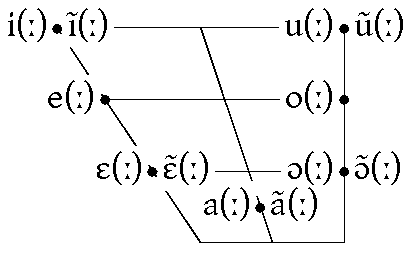
\includegraphics[width=0.4\linewidth]{figures/vowel}
	\caption{Vowel qualities}
	\label{fig:vowel}
\end{figure}

		%There are five phonemic oral and five nasal vowels, and lengthened counterparts:
	
	\begin{table}
		\caption{Minimal pairs for vowels}
		\fittable{\begin{tabular}{llll}
		\lsptoprule
			{[tʰi]} \qu{shell} & {[tʰiː]} \qu{pierce}& {[tɕuvi]} \qu{say standing} & {[tɕuːvi]} \qu{string up}  \\
			& {[wĩː]} \qu{strength} &&\\
			\midrule
			{[tʰe]} \qu{algae}&	{[tʰeː]} \qu{heavy}& {[so]} \qu{roof pole} & [soː] \qu{shoot (bot.)}\\
			{[tʰɛ̃]} \qu{limestone}&{[tʰɛ̃ːn]} \qu{run, fly} &{[tʰɔ̃a]} \qu{command}\footnote{Compare to /tʰo-a/ \qu{call-3\gl{sg}.\gl{obj}}}  &\\
			\midrule
			{[tʰa]} \qu{\gl{ass}}&{[tʰaː]} \qu{tie}&& \\
			{[tʰã]} \qu{feces}&&&\\
		\lspbottomrule
		\end{tabular}}
	\label{tab:phon}
	\end{table}

	
Apart from \textit{wîî} \qu{strength} vs alienable \textit{wii} \qu{field}, [ĩ] is not attested in minimal pairs, I thus treat it as a marginal vowel phoneme. The status of [ũ] is even trickier. 
%\subsection{The phonemic status of [ũ]}	
The nasal closed vowel [ũ] only appears in complementary distribution to its oral counterparts: after the aspirated consonants \textit{kh}, \textit{phw} etc discussed in \sectref{ssec:Aspiration}, after nasals, and in other nasalizing conditions. There are no long nasal vowels in open syllables at all (except [kʰĩː], which is still [kʰĩːk] in closely related Hmwaveke).
	Whether we analyze %/ĩ/ and 
	/ũ/ as a phoneme depends on our understanding of [kʰ]: 
	If [kʰ] is a phoneme, then %[ĩ/ and 
	[ũ] could be analyzed as an allophone of %/i/ and 
	/u/, conditioned by [kʰ]. %Arguments in favour of a phonemic status of [kʰ] are weak: firstly, other languages in the area have /k/ and [kʰ], and secondly, all other non-prenasalized plosives in Vamale have an aspirated phonemic counterpart. There are a few words, such as \textit{kholok} \qu{fall spontaneously} that can be elicited without a nasal vowel, but they are usually recent loanwords. If, on the other hand, we analyzede [kʰ] as a phonologically conditioned allophone  of [k] before nasal vowels, then %[kʰĩː/ \qu{swamp hen} and	[kʰũkʰũ] \qu{mute} is /kũkũ/, and /ũ/ is a marginal phoneme. Last possibility: /ũ/ is maintained in historically nasalized post-\textit{*kn} contexts, but without contrastive pairs, cannot be posited as a phoneme, regardless of the status of [kʰ], which is similarly unclear. 
This description will assume that the distribution of [ũ] is predictable, but will still transcribe [ũ] as \ort{û} except after nasals.
	
	\subsection{Quantity}
	\label{sec:VQuantity}
	\is{Vowels!Quantity}
	Vamale features phonemic length in both monosyllabic words, see the examples \textit{thi} \qu{shell} and \textit{thii} \qu{pierce} at the beginning of \sectref{sec:V} above, and polysyllabic ones.   %Campbell analyzes long vowels in monosyllabic words as underlying sequences of identical vowels in polysyllabic words: /tʰe.ep/ $\rightarrow$ [tʰɛːp] \qu{flow} \parencite[61]{campbell_phenomenon_1987}. This grammar does not. xxwhy not?
	
Consider the following minimal pairs:

\begin{itemize}
 \item\relax [ˈsa.m̥ʷã] \qu{go the other way} vs [ˈsaːm̥ʷã] \qu{banana}
 \item\relax [ˈfa.ti] \qu{language} vs [ˈfaː.ti] \qu{glue something}\footnote{The latter is morphologically complex: \textit{faat} \qu{be sticky} and \textit{-i} \qu{\gl{tr}}}
 \item\relax [ˈtʰa.ke] \qu{throw} vs [ˈtʰaː.ke] \qu{drag}
\end{itemize}
 
This analysis is contested for Voh-Koné languages: Campbell analyzes long vowels in Hmwaveke polysyllabic words as a feature of the stressed syllable \parencite[56]{campbell_phenomenon_1987}. In cases where a fortis-onset syllable takes the stress despite other factors, like the presence of a long syllable (e.g. [ˈtʰa.keː.ke] \qu{stretch out}), or a penultimate syllable (e.g. ['xaⁿ.ɟa.ke] \qu{eat starchy food}), this is argued to be due to extra articulatory energy, but not phonologically stress \parencite[59]{campbell_phenomenon_1987}.

In Vamale, however, many polysyllabic words are composed of only short syllables: e.g. \textit{'ta.na} \qu{ripe}, \textit{'xa.le.ke} \qu{see}, \textit{cu.va.'than.ke} \qu{stand apart}, \textit{'xa.ba.le} \qu{their mat}. Apart from lexical factors, length is conditioned by morphosyntactic factors as well. Possession
	%marked by the suffix \textit{-n} for open syllables, 
	will lengthen the final vowel of some directly possessed, alienable words:
	
	\begin{itemize}
		\item {[ˈfa.ti]} \qu{language} $\rightarrow$ {[fa.ˈtiːn]} \qu{language-3\gl{sg}.\gl{poss}}
		\item {[ˈiː.la]} \qu{cauldron} $\rightarrow$ {[iː.loːŋ]} \qu{my cauldron}
		\item \textit{ˈfʷaːn.dan} \qu{road} $\rightarrow$ {[ˌfʷan.da.ˈnũːŋ]} \qu{my road}
		%\item[/ \textit{}
	\end{itemize}
	
While quantity is phonemic, it is not always realized in everyday speech. Compare \textit{ju} \qu{fish kabob} to \textit{juu} \qu{real, sacred; very}. While the first word is only rarely produced nowadays,\footnote{The loanword \textit{brochette} being used to make the analytical \textit{brochette ko-n nyu} \qu{kabob with fish}} the latter is ubiquitous, and often in an unstressed position, or even a compound (see \sectref{sec:WCIntensifiers}). Both environments tend to elide stress, and unstressed long syllables are often shortened.	
	
\subsection{Quality}
\label{ssec:Vowel_Quality}
\is{Vowels!Quality}
The mid-open vowels have allophones depending on the syllable structure. Open syllables feature closed vowels. Closed syllables have several variables: closed short syllables feature the more open vowels [ɛ] and [ɔ]. Closed long syllables show both pairs; plosive-final syllables have more open vowels ([sɔːt] \qu{touch}), and nasal-final ones feature comparatively more closed vowels ([so̝ːm] \qu{swim}). See \Cref{tab:allovowels} for an illustration. Note that the vowels were rendered here without their nasalization: all vowels preceding nasals are to some degree nasalized, this does not affect with which allophone they are realized.
	
	\begin{table}
		\centering
		
		\caption{Vowel allophones in their defining contexts (nasalization omitted)}
		\begin{tabular}{lll}
			\lsptoprule
			&	[o]	[ɔ] &	[ɛ]	[e]\\
			\midrule
			V	&	[ˈpuːn.dɟo] \qu{whale}		&	[se] \qu{one}\\
			\midrule		
			Vː	&	[ˈtɕoː.lam] \qu{your part /to eat, to do]}		&	[seː] \qu{cry}\\
			\midrule		
			VC	&	[tɕɔp̚] \qu{pass over a ridge}&	[sɛp̚] \qu{coconut}	\\
			&	[ko.ˈkɔt̚] \qu{common mynah (bird)}&	[xɛt̚ ] \qu{warm}	\\
			%	[tʰilowɛc̚/ \qu{kind of tree}	
			&	[pʰɔm] \qu{butterfly}&	[fe.ˈtʰɛm] \qu{white spots (skin)}	\\
			&	[xɔŋ] \qu{my leg}&	[bɛŋ] \qu{waterfall}	\\
			&	[kɔn] \qu{\gl{prog}}&	[sɛn] \qu{poison}	\\
			\midrule		
			VːN	&	[mboːm] \qu{shade}		&	[ɣeːm] \qu{basket}\\
			&	[ɲa.ˈkoːn] \qu{for}		&	[xeːn] \qu{noise}\\
			&	[koːŋ] \qu{on me}		&	[mbeːŋ] \qu{my peer}\\
			\midrule				
			VːP	&	[ɣa.ˈkɔːp̚] \qu{wild}&	[tɛːp̚] \qu{flow (liquid)}	\\		
			&	[tɔːt̚] \qu{grass}, [ɔːt̚] \qu{rope; vein}&	[ˈtɛːt̚] \qu{be lazy}	\\
			\lspbottomrule
		\end{tabular}
		\label{tab:allovowels}
	\end{table}
	
	%Nêlêmwa has V: o and VC ɔ, with some exceptions in long (open and closed) contexts.
	
%	The mid-open vowels before nasals are more open than the ones before orals (compare /tʰe/ \qu{algae} and /tʰɛ̃/ \qu{rock}), meaning that the oral-nasal pairs are not all identical in their aperture.
	Possibly because the community is multilingual, there is considerable variation between individuals concerning the expression of nasality. Some nasalize almost all vowels that follow a nasal, which is why Rivierre does not consider nasality of vowels for Bwatoo, except after oral consonants \citeyearpar[25]{rivierre_bwatoo_2006}. %This conditioned nasalization is also found after the aspirated velar plosive [kʰ], see \Cref{ssec:Aspiration}.
	
	\subsection{Vowel sequences}
	\is{Vowels!Diphthongs}
	\begin{sloppypar}
	There are no diphthongs; recorded vowel sequences are either disyllabic or contain a glide, see \Cref{tab:v_sequences}. Some variants in fast speech seem to reduce the prominence of a syllable and make it approach an on- or offglide quality: /jo.a.kan/ [ˈⁿdɟoa̯.kãn] \qu{thick}.
	\end{sloppypar}
	

\begin{table}
\label{tab:v_sequences}
\begin{tabular}{lll}
\lsptoprule
	~ & Item & Translation  \\\midrule
	ie & [tʰi.en] & \qu{three} \\ 
	io & [ⁿɟi.ɔŋ] & \qu{my belly}  \\
		iu & [pi.uk] & \qu{star} \\ \addlinespace
	ia & [ci.a] & \qu{he is not there}  \\\addlinespace 
	ui & [bu̯i.ɲ̊o] & \qu{type of shell}  \\ 
	ue & [va.tu.e] & \qu{pick pandanus leaves}   \\ 
%uo & [tʰuːp] & shower & also uu, only one?!  \\ \addlinespace
	ua & [tʰu.a] & \qu{clear bush}   \\ \addlinespace
	ei & [pej.pa] & \qu{paper}  \\ 
	eu & [xe.u] & \qu{burn by neglect}  \\ 
	eo & [ⁿde.ɔŋ] & \qu{my spear}\\ 
	ea & [m̥ʷe.ap] & \qu{nest} \\ \addlinespace
	oi & [ᵐbʷa xo.lɔj] & \qu{wheel} \\ 
	oa & [ⁿɟo.a.kan] & \qu{thick}  \\ \addlinespace
	ai & [tʰaj] & \qu{roll up} \\ 
	ae & [mã.ẽ] & \qu{fire} \\ 
	ao & [ha.o] & \qu{grandfather}   \\ 
	au & [sa.ũn] & \qu{garment}  \\ \addlinespace
	uo & * & ~ \\ 
	oe & * & ~ \\ 
	ou & * & ~  \\ 
	\lspbottomrule
\end{tabular}
\caption{Vowel sequences with examples}
\end{table}
	%saun \qu{robe}
	
	\subsection{Allophones of vowels}
	\is{Vowels!Allophones}
Vowel allophony is underdescribed as of yet in Northern languages. Rivierre's detailed phonological description of Cèmuhî \citeyearpar[32, 35, 40]{rivierre_langue_1980} expands upon Haudricourt's brief account of the seven phonemic vowels \citeyearpar[373]{haudricourt_langue_1968}, and considers [ɔ] an allophone of /o/, amongst others. The phonology of the Hienghène languages was studied by \textcite{ozanne-rivierre_phonologie_1982}, but vowel allophones were not mentioned. Yuanga was described in detail by \textcite{schooling_phonology_1992}. There are no phonological descriptions focusing on vowel allophony for Nyelâyû \parencite{ozanne-rivierre_nyelayu_1998} and Nêlêmwa \parencite{bril_nelemwa_2002}.
 	
	\subsubsection{Nasalization of vowels}
	\label{ssec:NasalV}
	\is{Vowels!Nasalized vowels}
	Nasal spreading in both directions is described in detail for Hmwaveke \parencite[66, 76]{campbell_phenomenon_1987}. Vamale has this, too, and both regressive (e.g. [nĩũ] \qu{fish}, (\ref{ex:Vass})) as well as progressive assimilation (e.g. [ãmbu] \qu{\gl{1}\gl{du}.\gl{excl}}, see ex. \ref{ex:Vass2}) to nasals are so frequent that nasality of vowels is most often not phonemic.
	

\ea\label{ex:Vass} 		
[fetãmɛ̃]\\
\gll fe-ta-me\\
		 take-move.up-\gl{dir.cp}\\
\glt \qu{bring up} 
\z


\ea\label{ex:Vass2}
[fɛ̃ãmɛ̃]\\
\gll fe-hân-me\\		
 take-move.same.level-\gl{dir.cp}\\		
\glt \qu{bring (across the same plain)}
\z



	
	%Vowels are often nasalized after nasal consonants, as in Bwatoo \parencite[25]{rivierre_bwatoo_2006}. 
	Nasality also spreads from one vowel to another (regressive assimilation), but does not seem to do so across oral consonants, see (\ref{ex:Vass}). Spreading of nasality is so prevalent in Hmwaveke that Campbell considers it a word-level feature, and that words with truly phonemic nasal vowels are only those that have, among other factors: \begin{enumerate}
		\item no nasal or semi-nasal consonants
		\item and a nasal vowel in the stressed syllable \parencite[66]{campbell_phenomenon_1987}
	\end{enumerate}
	Like nasal vowels, nasalized ones are usually realized more open than their oral counterparts, i.e. /e/ and /o/ are realized as [ɛ̃] and [ɔ̃], respectively. %While nasal /ã/ the vowel in \textit{han} \qu{to walk, to go} is, due to the final nasal, often pronounced [hæ̃n]. 

	
	\subsubsection{Fronting of /u/}
	\label{ssec:fronting_u}
	/u/ is frequently, but not always, fronted to [y] or [ʏ] after the front %(\textbf{	Do you mean immediately after, or in a syllable following a syllable with /i/?})
	 vowel /i/ and its non-syllabic variant [j] (\ref{ex:nyayung}, \ref{ex:xayu}). When asked to pronounce the word as slowly as possible, some speakers like Jaaun Kalène produced [ˈɣaː.e.ʉ] or something further front, while others, like Elise Oué, would have two syllables [ˈɣa.ju]. The latter form is likely to be underlying, as the Pije cognate \textit{ka.hyuk} \parencite[135]{haudricourt_dictionnaire_1982} %and Cèmuhî /áíú/ \parencite[148]{rivierre_langue_1980} suggest a lenition of initial /k/, dropping of final /k/, and a glide between the vowels /a/ and /u/. 
	 suggests that two syllables, with a glide as the second onset, are etymological. While this fronting is not described by Ozanne-Rivierre for Pije, she mentions it for Jawe, as having developed after an intervocalic /v/ was dropped: /ʏi/ \qu{blow} (cf. \textit{uvi} in Fwâi and eastern Nemi) \citeyearpar[22]{ozanne-rivierre_phonologie_1982}. %In Vamale, {[}uŋ] is the allomorph of -\textit{ong} \qu{1\gl{sg}.\gl{poss}} after /i/. This is lexicalized in inalienable lexemes whose stem ends on -\textit{i} (/si-ong/ [sũŋ]\goodtilde[sʏ̃ŋ] \qu{my hand}, /jati-ong/ [ɟatuŋ] \qu{my younger sibling}), but occurs sporadically with other words. A similar phenomenon is described for Nyelâyu \parencite[25]{ozanne-rivierre_nyelayu_1998}, where a realization of /we/ as [ø] in is also discussed.%xhüüli in Kito 
	
	
	\ea\label{ex:nyayung}
%	\ili{}{}{ \textit{nyayung}}
	[ɲãʏ̃ŋ] \goodtilde [ɲãjuŋ]\\
	\gll nyai-ong\\	
	 child-1\gl{sg}.\gl{poss}\\
		\glt \qu{my child}
	\z
	
	
	\ea\label{ex:xayu}
	[ɣaːʏ] \goodtilde [ɣaːju̹]\\
	\gll xayu \\ %\footnotemark\\
	male \\
	\glt \qu{boy, male}
	\z
	
%	\footnotetext{Pije cognate \textit{kahyuk} \qu{man}}
	
	\subsubsection{Backing and rounding of /a/}
	
	/a/ is often backed and centralized in progressive assimilation to labiovelar approximants, a phenomenon also described for Yuanga \parencite[129]{schooling_phonology_1992}. This happens most frequently with \textit{vwa} \qu{do; exist}, especially where it is part of a compound, e.g. \ort{vwa wîîn} [wɒ wĩːn]  \goodtilde [wo wĩːn] \qu{\gl{exist} strength} \qu{be strong}. This is not found in careful pronunciation, but is a regular allophone in Hmwaveke \parencite[16]{campbell_phenomenon_1987}.%, suggesting the phenomenon is at least a century old.
	
%	\subsubsection{Fronting and raising of /a/}
%	
%	
	
	\subsubsection{Interplay between /a/ and \textit{e=} \qu{1\textsc{sg}}}
	
	Some morphemes ending with /a/ will assimilate to the 1\gl{sg} subject index \textit{e=} (\ref{ex:the}). As examples (\ref{ex:cama}) and (\ref{ex:ceme}) show, this process can spread over at least one more syllable, though this depends on the speaker.
	
	\ea
	\label{ex:the}
	(\textit{the bwa han})\\
	\gll tha=e=bwa hân\\
	 \gl{ass}=1\gl{sg}=\gl{ipfv} go\\
	\glt \qu{I am leaving}
	\z
	
	\ea\label{ex:cama}
	(\textit{nyiman cama go vwa})\\
	\gll nyima-n (ca)ma go=vwa\\
	 want-3\gl{sg} \gl{subr} 2\gl{sg}=do\\
	\glt \qu{He wants you to do it.}
	\z
	
	\ea\label{ex:ceme}
	(\textit{nyiman ceme vwa})\\
	\gll nyima-n cam=e=vwa\\
	 want-3\gl{sg} \gl{subr}=1\gl{sg}=do\\
	\glt \qu{He wants me to do it.}
	\z
	
%	\a
%	
%	\ili{}{}{} \textit{tha go hân}
%	\gll tha go hân
%	 \gl{ass}=2\gl{sg} go
%	\glt \qu{You go}
%	
	

	
%	\a
%	
%	\ili{}{}{} cipe caihnan li=aman a go vi
%	\gll cipa e=caihna-n li=aman a go=vi	
%	 \gl{neg} 1\gl{sg}=know-\qu{tr} \gl{def}.\gl{pl}=thing \gl{rel} 2\glsg}=say
%	\glt \qu{I don't know the things you said}
%	
%	
%	
%	\a
%	
%	\ili{}{}{} cipa go caihna-n li=aman \textbf{e} vi
%	\gll 	cipa go caihna-n li=aman a e=vi	
%		\gl{neg} 2\glsg} know-\qu{tr} \gl{def}.\gl{pl}=thing \gl{rel} 1\gl{sg}=say
%	\glt	\qu{You don't know the things I said}	
%	
	
	%Bril thinks this is si-ong with o getting raized, because it overrides the previous vowel in xha-ong . no known reason why only a should suffer. e- because distinctive and the language avoids diphthongs. 
	
	Vamale is the only Voh-Koné language described with this assimilation of /a/ to the first person subject index \textit{e=}. The sequence [ae] appears elsewhere in the language without assimilating (e.g. [ɣa.ˈm̥ã.ɛ̃n] \qu{tomorrow}); the assimilation is specific to the subject marker. It is also noteworthy that this subject marker only occurs in Vamale within Voh-Koné. While neither Hmwaveke nor Pije \parencite[246, 247]{haudricourt_dictionnaire_1982} have subject marker proclitics that differ from the free form, Cèmuhî has a pair /(wa)eo/ vs. /e/ \parencite[61]{rivierre_langue_1980}; Vamale may have borrowed \textit{e=} \qu{1\gl{sg}} from it. The assimilation, however, is not described for Cèmuhî either.
	
	\section{Phonotactics/syllable structure}
	\is{Syllable structure}
	%Contrary to other described Voh-Koné languages, Vamale allows exactly one cluster:
	%\textit{xhwatla} \qu{thunder}. Its cognates are \textit{xhwalaa} in Bwatoo and \textit{xhwala} in Tiéta. A form /xʷalala/ is present in Hmwaveke and could be a preceding form. POc *kuru
	\begin{sloppypar}
	Like its Hienghène and Voh-Koné relatives, Vamale exhibits a (C(ʰʷ))V(VVC) syllable pattern. Pre-nasalized consonants preceded by a vowel (e.g. V\# \#ⁿC, or V.ⁿC) are reanalyzed, and their nasal is assigned to the preceding syllable: /abu/ /am.bu/ \qu{1\gl{du}.\gl{excl}}. %Offglides could be 
	Consonants usually meet at morpheme boundaries, like [wan.ke] \qu{change}, /bofwa-n-mwa/ [bo.fʷan.mʷã] \qu{door, door-of-house}. The only exception found is the morphologically simple word /xʷat.la/ \qu{thunder}, still /xʷa.la.la/ in western varieties.\footnote{In this case, the second syllable /la/ was likely reduced and the cluster fortized to /l̥/, before being split into a stop and a glide.ˈ Most morphologically simple words have one or two syllables.}
	\end{sloppypar}
	
	\section{Reduplication}
	Reduplication is a common morphological process in many Oceanic languages, but plays a negligible role in Vamale. Historically, most old CVCV reduplications, probably already stripped of their morphological function, developed first into CCV geminates through elision of the first syllable's vowel, and then into aspirated plosives or voiceless fricatives (see \sectref{ssec:Aspiration}). Since productive derivational processes work with prefixes%(see \sectref{sec:NomDeriv})
	, the following forms are probably not representative of productive processes.
	\is{Reduplication}
	\is{Negation}
	%Kakai, more polite form of kai \qu{who}
	
	\begin{itemize}
		\item \textit{kokoi}, polite negation, loan from Pije (where \textit{koi} is the negation)
		\item \textit{hahat} \qu{nono}, from \textit{hat} \qu{strong negation}
		\item \textit{sisipo}, \qu{together}, \textit{nya-sipo-ke} \qu{put-together-\gl{tr}}
		\item \textit{fwafwa} \qu{full of holes}, from \textit{fwa} \qu{hole}
		\item \textit{juuju(u)} \qu{truth}, from the root \textit{juu} \qu{true}
		\item \textit{vayavaya} \qu{shaky}, from \textit{vaya} \qu{move}
	\end{itemize}
	
	%xaxahnang \qu{beautiful}, possibly? xa- is a nominalizer but xahnang is maybe not a nominalisable verb? xa- is also a habitual.
	
	\section{Stress}
	\label{sec:Stress}
	\label{sec:stress}
	\is{Stress}
	In Vamale, disyllabic words have penultimate stress, as is typical in Oceanic settings. Trisyllabic, morphologically simple, non-derived nouns take stress on the first syllable, see \Cref{tab:tri}. These are rare, though loanwords now increase their number.

\begin{table}
\caption{Stress in trisyllabic words}
\label{tab:tri}
\begin{tabular}{ll}
\lsptoprule
	Old words & Loanwords\\\midrule
{[}ˈa.pu.li] \qu{person} & {[}ˈᵐbu.ɾu.(w)ɛt] \qu{wheelbarrow},\\
                         & \quad from French [bʁu.ˈɛt]\\
{[}ˈva.ma.le]\qu{vamale}&{[}ˈmãŋ.ga.sĩ] \textasciitilde {[}maŋ.ga.ˈsî/ \qu{shop},\\
                         & \quad  from French {[}magaˈzĩ]\\
{[}ˈⁿdon.dam.ba] \qu{flood garbage}&{[}ˈpu.a.ka] \qu{pig},\\
                         & \quad  from Polynesian \textit{puaka}\\
{[ˈma.vu.lɛn]} \qu{flying fox sp.}&  {[ˈku.mʷa.la]} \qu{sweet potato},\\
                         & \quad  from Polynesian  \textit{kumala}\\
{[ˈma.tʰi.la]} \qu{small bird sp.}&{[}ˈᵑge.ɾe.nũ] \qu{frog},\\
                         & \quad from French \textit{grenouille}\\
\lspbottomrule
%	\item {[ˈⁿdom.bin.do]}  \qu{mangrove eel}
%\item {[ˈpʷa.la.lu]} \qu{rainbow}

%	\item {[}ˈla.lu.ɛn/ \qu{aloe plant}, from French /laloˈɛs]
\end{tabular}
\end{table}

Longer words are morphologically complex and have stress on the penultimate stress-bearing unit, which is often a syllable of the root, but not always. While some morphological factors complicate the picture, regular phonological aspects predict most stress positions. A closed syllable will be stressed over an open one, a fortis onset will usually top a tenuis onset, and a long syllable will be stressed above all else. This gives us a hierarchy of factors:

\ea Long syllable > fortis onset > closed syllable > penultimate syllable
\z
	
%	\begin{table}
%		\label{tab:stress}
%		\caption{Examples for stress in various contexts}
%		\begin{tabular}{lllll}
%			&	\multicolumn{2}{c}{Mono-morphemic}		&\multicolumn{2}{c}{Poly-morphemic}		\\
%			\midrule
%			\multirow{3}{2cm}{open syllable (short)}	&	{[ˈpa.la]} &\qu{speak}		& /ˈpa.la.ke]& \qu{speak /a language]}		\\
%			&	{[ˈfa.to]} &\qu{drink warm}		& /ˈfɛ̃.ã.nã.ke/ &\qu{show}	\\
%			%&	{[ˈfa.va]} &\qu{four}&  &\\
%			\midrule		
%			\multirow{3}{2cm}{open (syllable (long))}	&	{[ˈsaː.m̥ãt]} &\qu{fog}	&	[fu.ˈnãː.ke/ &\qu{preach}			\\
%			& {[ɣe.ˈtʰoː]} &\qu{landing net} & /ˈɣa.fu.nã]& \qu{middle finger (lit. \qu{preacher})}\\
%			& {[ˈmãː.vu]} & \qu{close eyes} &&\\
%			\midrule
%			\multirow{3}{2cm}{closed syllables (short)}&	{[ˈɣaⁿ.ɟe]} &\qu{eat.juicy}  	& /ˈɣa.le.lu/ &\qu{see them}		 \\		
%			&	{[ˈm̥aw.tɕɛp]}& \qu{noni tree}& &		\\	
%			&	{[ˈuⁿ.du]} &\qu{drink cold}&&\\
%			
%			\midrule		
%			\multirow{3}{2cm}{closed syllables (long)}&{[ɣa.ˈkɔːp]}& \qu{wild}&[ɲãˈkõ:ŋ/ &\qu{for me}	\\
%			&{[te.mĩ.ˈnɛ̃ːn]} & \qu{float}& /si.nũ.ˈxiːt]& \qu{painful suffering}\\
%			&{[xa.ˈsaːt]} & \qu{jump}& /fa.ˈto̟ːm]&\qu{your drink}\\
%			\midrule
%			\multirow{4}{2cm}{3 syllables}& 	{[fʷaⁿ.ˈɟi.mʷã]}&\qu{ask}	&	[fʷaⁿ.ˈɟi.mʷã.ke]&\qu{ask (\gl{tr})}	\\
%			&	{[ˈpu.a.ka]} &\qu{pig}	&	[pu.a.ˈka.nɛ̃ɔ̃ŋ/ &\qu{my pig} \\
%			&	{[ˈtʰɔ.a.tit]}& \qu{sky}	&	{[ˈtʰɔ.a.tit̚.tɕa]}	& \qu{this day}\\
%			&   {[pu.ˈpʷaː.le]}& \qu{European} &	[pa.ˈpan.go/ &\qu{your father} \\
%			&	{[tʰe.ˈxʷaːⁿ.de]}& \qu{Tiouandé village}	&[ˈɣaᵐ.bu.na]& \qu{thief}				\\
%			&  {[ˈpʷa.la.lu]} & \qu{rainbow} & & \\
%		\end{tabular}
%		
%	\end{table}
%	

% 	\label{ssec:compF}
\is{Stress!Extrametrical morphemes}
\is{Stress!Complicating factors}
	Some monosyllabic morphemes do not count in the stress pattern. One frequent example is the extrametrical suffix \textit{-ke} \qu{\gl{tr}}, whose phonological non\hyp importance makes the third syllable in /fʷan.ˈɟi.mʷa.ke/ \qu{ask something} the penultimate of the phonological word. %\textit{-ke} may be related to the proclitic \textit{ka} which marks subjects and possessors. 
	Possessive and object-indexing suffixes shift the stress, but not in a simple syllable-counting way, as [ˈᵐbwãn.ɟɛp], [ᵐbwãn.ˈɟɛp.go] \qu{hand drum, hand drum-2\gl{sg}.\gl{poss}} would suggest, i.e. with the stress, all other things being equal, moving to the new penultimate syllable. However, since \textit{bwajep-gavwe} [ˌᵐbwãn.ˈɟɛp.ga.vʷe] \qu{hand drum-2\gl{pl}.\gl{poss}} does not have the stress on the penultimate syllable of the phonological word, [ga], this suggests an analysis of root syllables that is different from that of suffixed morphology. Possessive and object-indexing suffixes count as a single unit in stress assignment, meaning that a two-syllable possessive suffix such as \textit{-gavwe} \qu{2\gl{pl}.\gl{poss}} has the same effect as \textit{-go} \qu{2\gl{sg}.\gl{poss}}.
	
	Speech act participant indexes (the proclitics, not the suffixes) are also extrametrical: 
	
	\begin{itemize}
		\item  /ˈɣa.le.ke/ \qu{to see}
		\item /le=ˈɣa.le-le/ \qu{3\gl{pl}=see-3\gl{pl}.\gl{obj}}, \qu{they see them}
		\item  /le=ɣa.le-ˈkaː.vʷe/ \qu{they see you}, also pronounced /le=ɣa.ˈle.ka.vʷe/ 
	\end{itemize}
%In verbs with long stem vowels, the 
%	%[fʷaⁿ.ˈɟi.mʷa]
%	%fa.ˈlɔŋ.ga.vi
%	[ˈxʷiː.ko]
%	[ˈxʷiː.le]
%	[ˈxʷiː.kavʷe]
\begin{sloppypar}
Other syllables attract stress. The nominalizer \textit{xa-} \qu{\gl{agt}.\gl{nmlz}} (from \textit{xayu} \qu{male}) always attracts stress (probably due to its etymology, see \sectref{ssec:agt.nmlz}), but not the nominalizers \textit{hun-} \qu{manner.\gl{nmlz}} nor \textit{ape-} \qu{place.\gl{nmlz}} (from \textit{ape-n} \qu{trace}).
\end{sloppypar}
	
\begin{table}
		\begin{tabular}{ll}
		{[ˈhun.vʷa ]} \qu{way of doing}&{[a.ˈpe.ta]} \qu{ladder (place of going.up)}\\
		{[hun.ˈmõː]} \qu{way of living}&{[a.pe.ˈmõː]} \qu{dwelling}\\
	\end{tabular}
\end{table}

Semantically bleached function words like /a.ˈman/ \qu{thing; object place-holder} are re-analyzed as one foot in compounds: 
	
	%[ˈxʷi.ja.mãn/ \qu{eat}
\begin{itemize}
	\item {[}ˈtɕaj.n̥ãn] \qu{know}, [tɕaj.ˈn̥ãn.ã.mãn] \qu{know something}
	\item {[}ˈtɕãm.bi] \qu{smash}, [e.tɕãm.ˈbi.jã.mãn]  \qu{hammer}
\end{itemize}
	
The complex word \textit{ape-caihnan-aman-le}, \qu{\gl{nmlz}-know-thing-3\gl{pl}.\gl{poss}} \qu{their knowledge}, is pronounced {[ˌa.pe.tɕaj.n̥ãn.ã.ˈmãn.le]} by Kaina Fouan, which could be explained by analyzing \textit{(ape-)caihnan-aman} \qu{(fact.of-)know-thing} as a compound, \textit{-le} \qu{3\gl{pl}.\gl{poss}} as a suffix, and thus the main stress would fall on the penultimate syllable.
	%The stress seems to be on the root in a complex word, on long vowels, and to be penultimate
	
	%\todo{Find out which words have long vowels}
	%stress in Yuanga is penultimate d.h. calculated from ]#, 
	%intonation is trochäus, 
	%one syllable can contain 2 morae, syllable weight attracts stress
	%accent of trisyyl is on first syll if strong onset energy "attaque", dh aspirated plosives and h
	%composites have different stress but not the verbal tha-, co- things
	
%	\subsubsection{Related languages, their analysis, and how it relates to mine}
For Hmwaveke, stress is described as being fundamentally penultimate \parencite[59]{campbell_phenomenon_1987}, and forms which deviate from this, with few exceptions, are analyzed by Campbell as several phonological words. Campbell analyzes long syllables in plurisyllabic words as resulting from stress (suggesting that, fundamentally, length is a feature of all stressed syllables). For Vamale, though long syllables are stressed, I argue that the relation is reversedː length attracts stress.
 
In Nêlêmwa, stress is usually on the first syllable of the lexical root \textit{kâ-ˈyuva} \qu{how is it? (lit. lying.down-be.thus)} \parencite[26]{bril_nelemwa_2002}. This correlation between morphological structure and stress pattern is mirrored in Vamale to a certain extent, in that bound morphemes such as \textit{e-} \qu{\gl{recp}}, \textit{-ke} \qu{\gl{tr}}, and manner prefixes like \textit{mi-} \qu{do lying down} do not affect the position of the main stress. %The reduplicated form \textit{sisipo} \qu{do together} from \textit{sipo}, still found in \textit{nya-sipo-ke} \qu{put-together-\gl{tr}} is stressed on the first syllable instead of the second, 

	

%	\begin{table}
%		\label{tab:stress}
%		\caption{Examples for stress in various contexts}
%		\begin{tabular}{lllll}
%			&	\multicolumn{2}{c}{Mono-morphemic}		&\multicolumn{2}{c}{Poly-morphemic}		\\
%			\midrule
%			\multirow{3}{2cm}{open syllable (short)}	&	{[ˈpa.la]} &\qu{speak}		& /ˌlu.e.ˈpa.la]& \qu{they speak to each other}		\\
%			&	{[ˈfa.to]} &\qu{drink warm}		& /ˈfɛ̃.ã.nã.ke/ &\qu{show}	\\
%			&	{[ˈfa.va]} &\qu{four}&  &\\
%			\midrule		
%			\multirow{3}{2cm}{open (syllable (long))}	&	{[ˈsaː.m̥ãt]} &\qu{fog}	&	[fu.ˈnãː.ke/ &\qu{preach}			\\
%			& {[ɣe.ˈtʰoː]} &\qu{landing net} & /ˈɣa.fu.nã]& \qu{middle finger (lit. \qu{preacher})}\\
%			& {[ˈmãː.vu]} & \qu{close eyes} &&\\
%			\midrule
%			\multirow{3}{2cm}{closed syllables (short)}&	{[ˈɣaⁿ.ɟe]} &\qu{eat.juicy}  	& /ˈɣa.le.lu/ &\qu{see them}		 \\		
%			&	{[ˈm̥aw.tɕɛp]}& \qu{noni tree}& &		\\	
%			&	{[ˈuⁿ.du]} &\qu{drink cold}&&\\
%			
%			\midrule		
%			\multirow{3}{2cm}{closed syllables (long)}&{[ɣa.ˈkɔːp]}& \qu{wild}&[ɲãˈkõ:ŋ/ &\qu{for me}	\\
%			&{[te.mĩ.ˈnɛ̃ːn]} & \qu{float}& /si.nũ.ˈxiːt]& \qu{painful suffering}\\
%			&{[xa.ˈsaːt]} & \qu{jump}& /fa.ˈto̟ːm]&\qu{your drink}\\
%			\midrule
%			\multirow{4}{2cm}{3 syllables}& 	{[fʷaⁿ.ˈɟi.mʷã]}&\qu{ask}	&	[fʷaⁿ.ˈɟi.mʷã.ke]&\qu{ask (\gl{tr})}	\\
%			&	{[ˈpu.a.ka]} &\qu{pig}	&	[pu.a.ˈka.nɛ̃ɔ̃ŋ/ &\qu{my pig} \\
%			&	{[ˈtʰɔ.a.tit]}& \qu{sky}	&	{[ˈtʰɔ.a.tit̚.tɕa]}	& \qu{this day}\\
%			&   {[pu.ˈpʷaː.le]}& \qu{European} &	[pa.ˈpan.go/ &\qu{your father} \\
%			&	{[tʰe.ˈxʷaːⁿ.de]}& \qu{Tiouandé village}	&[ˈɣaᵐ.bu.na]& \qu{thief}				\\
%			&  {[pʷa.la.lu]} & \qu{rainbow} & & \\
%		\end{tabular}
%		
%	\end{table}
	
	%['xa.wa.xan/ dog or /xa.wa.'xan]?
	%[doː.'hã:/ curry ?
	
